% -------------------------------
% Plantilla del TFM en la ESIIAB/ESICR de la UCLM. Versión 0.1 (Preliminar)
%
% Luis de la Ossa
% 
% Compilar con XeLaTeX 
% -------------------------------
\documentclass[12pt, a4paper]{book}

% -------------------------------
% Información y opciones del documento. Debe editarse.
% -------------------------------
% -------------------------------
% Plantilla del TFM en la ESIIAB/ESICR de la UCLM. Versión 0.1 (Preliminar)
%
% Luis de la Ossa
% 
% Compilar con XeLaTeX 
% -------------------------------


% -------------------------------
% Comandos comunes
% -------------------------------
\newcommand{\uclm}{Universidad de Castilla-La Mancha\,}
\newcommand{\dsi}{Departamento de Sistemas Informáticos\,}
\newcommand{\esii}{Escuela Superior de Ingeniería Informática de Albacete\,}
\newcommand{\esi}{Escuela Superior de Informática de Ciudad Real\,}
\newcommand{\iiia}{Instituto de Investigación en Informática de Albacete\,}


% -------------------------------
% Comandos específicos
% -------------------------------
\newcommand{\autor}{Raúl Bernalte Sánchez\,}
\newcommand{\titulo}{Automatización inteligente de Protocolo para el Análisis de Muestras de Lenguaje Asistido en SAAC\,}
\newcommand{\director}{Nombre del director\,}
\newcommand{\codirector}{Nombre del codirector\,}
\newcommand{\fecha}{Julio, 2025\,}
 \newcommand{\espec}{Tecnología específica\,} 







% -------------------------------
% Configuración del documento, paquetes, etc. 
% -------------------------------
% -------------------------------
% Plantilla del TFM en la ESIIAB/ESICR de la UCLM. Versión 0.1 (Preliminar)
%
% Luis de la Ossa
% 
% Compilar con XeLaTeX 
% -------------------------------


% -------------------------------
% Idioma
% -------------------------------
\usepackage{polyglossia}
\setmainlanguage{spanish}


% -------------------------------
% Fuente
% -------------------------------
% Cualquier tamaño de texto: {\fontsize{100pt}{120pt}\selectfont tutexto}
\usepackage{anyfontsize}
% Selección de fuentes.
\usepackage{fontspec}
% Espacio entre líneas
\usepackage{setspace}
% Fuentes especiales
\usepackage{textcomp,marvosym,pifont}


% -------------------------------
% Otros paquetes de uso común
% -------------------------------
% Símbolos matemáticos
\usepackage{amsmath,amsfonts,amssymb}
% Gráficos
\usepackage{graphicx}
% Posición arbitraria de los gráficos
\usepackage[absolute,overlay]{textpos}
% Apéndices
\usepackage{appendix}


% -------------------------------
% Esquema de colores
% -------------------------------
% Paquete para la definición de colores
\usepackage[table]{xcolor}
% Esquema de colores
% -------------------------------
% Plantilla del TFM en la ESIIAB/ESICR de la UCLM. Versión 0.1 (Preliminar)
%
% Luis de la Ossa
% 
% Compilar con XeLaTeX 
% -------------------------------

% -------------------------------
% Color del tema
% -------------------------------

% Color para los títulos, etc.
\definecolor{tema}{RGB}{0,0,0}            % Negro (Recomendado)
%\definecolor{tema}{gray}{.50}            % Gris 50
%\definecolor{tema}{RGB}{183, 18, 52}     % LOGO UCLM
%\definecolor{tema}{RGB}{31, 78, 121}     % Azul del esquema  
%\definecolor{tema}{RGB}{153, 61, 61}     % Rojo del esquema     

% Negritas con el color del tema
\newcommand{\bft}[1]{\textcolor{tema}{\bf #1}} 


% -------------------------------
% Esquema de colores
% -------------------------------
% Se pueden redefinir para que coincidan con las paletas de las 
% herramientas utilizadas para hacer las gráficas.
\definecolor{blanco}{RGB}{255,255,255} 
\definecolor{negro}{RGB}{0,0,0}
\definecolor{gris95}{gray}{.95}
\definecolor{gris75}{gray}{.75}
\definecolor{gris50}{gray}{.50}
\definecolor{gris25}{gray}{.25}
\definecolor{rojo}{RGB}{153, 61, 61}        
\definecolor{uclm}{RGB}{183, 18, 52}       % Corporativo UCLM
\definecolor{azul}{RGB}{31, 78, 121}       
\definecolor{verde}{RGB}{82, 112, 87}      
\definecolor{naranja}{RGB}{196, 118, 58} 
\definecolor{mostaza}{RGB}{179, 147, 63} 

% Negrita con color definido 
\newcommand{\bfa}[1]{\textcolor{azul}{\bf #1}} 
\newcommand{\bfr}[1]{\textcolor{rojo}{\bf #1}}
\newcommand{\bfn}[1]{\textcolor{naranja}{\bf #1}}
\newcommand{\bfv}[1]{\textcolor{verde}{\bf #1}}  
\newcommand{\bfm}[1]{\textcolor{mostaza}{\bf #1}} 






% -------------------------------
% Márgenes
% -------------------------------
% Márgenes de las páginas
\usepackage[
  inner	 =	3cm,   % Margen interior
  outer	 =	2.5cm, % Margen exterior
  top	 =	2.5cm, % Margen superior
  bottom =	2.5cm, % Margen inferior
  includeheadfoot, % Incluye cabecera y pie de página en los márgenes
]{geometry}

% Muestra una regla para comprobar el formato de las páginas (descomentar)
%\usepackage[type=upperleft,showframe,marklength=8mm]{fgruler} 


% -------------------------------
% Interlineado
% -------------------------------
\usepackage{setspace}
\onehalfspacing    % interlineado 1.5
%\doublespacing     % interlineado doble
%\singlespacing     % normal


% -------------------------------
% Renombra tablas y bibliografía
% -------------------------------
\addto\captionsspanish{
	\renewcommand{\listtablename}{Índice de tablas} 
	\renewcommand{\tablename}{Tabla}
	\renewcommand{\bibname}{Referencia bibliográfica}
}


% -------------------------------
% Itemize y enumerate. Control de los espacios.
% -------------------------------
\usepackage{enumitem}
\setitemize{itemsep=0pt}
\setenumerate{itemsep=0pt}
\renewcommand{\labelitemi}{\tiny\bft{$\blacksquare$}}
\renewcommand{\labelitemii}{\bft{$\bullet$}}
\renewcommand{\labelitemiii}{\bft{-}}


% -------------------------------
% Enlaces y colores
% -------------------------------
\usepackage{hyperref}
%\hypersetup{
%    colorlinks,
%    citecolor=black,
%    filecolor=black,
%    linkcolor=black,
%    urlcolor=black
%}

% -------------------------------
% Gestión de elementos flotantes
% -------------------------------
% Para forzar a que las figuras aparezcan antes del fin de una sección.
%\usepackage[section]{placeins}

% Gestión de títulos de los elementos flotantes
\usepackage{caption}
% Subfiguras y títulos en subfiguras
\usepackage{subcaption}

% Títulos
\DeclareCaptionFont{tema}{\color{tema}} % Color
\captionsetup{labelfont={tema, bf}}     % Estilo
\captionsetup{font=normalsize}          % Tamaño
\captionsetup{width=.9\linewidth}       % Anchura del título
 % Distancia de la figura al texto.
\setlength{\intextsep}{1cm} 
\setlength{\textfloatsep}{1cm}         
       

% -------------------------------
% Utilidades para tablas
% -------------------------------
% Para fundir filas en tablas
\usepackage{multirow}
% Para definir columnas con ancho fijo y alineación
\usepackage{array,ragged2e}
\newcolumntype{L}[1]{>{\raggedright\let\newline\\\arraybackslash\hspace{0pt}}m{#1}}
\newcolumntype{C}[1]{>{\centering\let\newline\\\arraybackslash\hspace{0pt}}m{#1}}
\newcolumntype{R}[1]{>{\raggedleft\let\newline\\\arraybackslash\hspace{0pt}}m{#1}}


% -------------------------------
% Para tabular
% -------------------------------
\usepackage{tabto}


% -------------------------------
% Formato de títulos, capítulos, etc.
% -------------------------------
\usepackage{titlesec, titletoc}
% Parte
\titleformat{\part}[display]												     	   % Estilo
	{\Huge \centering \color{tema}}                                                % Formato
	{Parte \thepart }                                                              % Etiqueta
	{0.75ex}                                                                       % Separación
	{\bfseries\fontsize{25pt}{40pt}\selectfont}                                    % Entre etiqueta y título            
	[\thispagestyle{empty}]                                                        % Después

% Capítulo		
\titleformat{\chapter}[block]            			 			                    % Estilo  	
	{\vspace{0cm} \flushright \bfseries \LARGE \color{tema}}  	        		% Formato 
	{\thechapter.}                  			  									% Etiqueta
	{0.75ex}                                     									% Separación
	{}                                           									% Entre etiqueta y título
	[\vspace{-0.25cm} \rule{0.5\textwidth}{1pt}\vspace*{1cm}\thispagestyle{plain}]    % Después      
  
% Sección
\titleformat{\section}
	{\vspace{5pt}  \Large \color{tema}}
	{\thesection .}
	{0.75ex}
	{}

% Subsección
\titleformat{\subsection}
	{\large \color{tema}}
	{\thesubsection .}
	{0.75ex}
	{}
 
% Subsubsección
\titleformat{\subsubsection}
	{\bf\color{tema}}
	{}
	{0.75ex}
	{}
	 
% Parte (TOC)
\titlecontents{part}[2pc]
  	{\vspace{20pt}\bfseries\filright\Large\color{tema}}
  	{\contentslabel{1.5pc}}{\hspace*{-1.5pc}}
  	{\vspace{5pt}}
  	{}
  
% Capítulo (TOC)
\titlecontents{chapter}[2pc]
  	{\vspace{10pt}\bfseries\large\filright}
  	{\contentslabel{1.5pc}}{\hspace*{-1.5pc}}
  	{\mdseries\titlerule*[0.5pc]{.}\bfseries\contentspage}

% Sección (TOC)
\titlecontents{section}[4pc]
  	{\vspace{5pt}\filright}
  	{\contentslabel{2pc}}{\hspace*{2pc}}
  	{\titlerule*[0.5pc]{.}\contentspage}
  	{\vspace{5pt}}

% Subsección (TOC)
\titlecontents{subsection}[6pc]
  	{\vspace{2.5pt}\filright\small\em}
  	{\contentslabel{3pc}}{\hspace*{-3pc}}
  	{\titlerule*[0.5pc]{.}\contentspage} 
  	
  	
% -------------------------------
% Cabeceras y pie de página
% -------------------------------
\usepackage{fancyhdr}
\pagestyle{fancy}
\fancyhf{}

% Permite incluir la parte. Para ello crea \parttitle
\let\Oldpart\part
\newcommand{\parttitle}{}
\renewcommand{\part}[1]{\Oldpart{#1}\renewcommand{\parttitle}{#1}}

% Cabeceras y pies de página
\fancyhead[LE]{}
\fancyhead[RO]{\slshape \leftmark}
\fancyfoot[LE,RO]{\thepage}
\renewcommand{\footrulewidth}{1pt}
\renewcommand{\headrulewidth}{1pt}
\renewcommand{\chaptermark}[1]{\markboth{#1}{}} % Capítulo (Solo texto)
\renewcommand{\chaptermark}[1]{\markboth{\thechapter. #1}{}} % Capítulo (Número y texto)

% Formato plano para las páginas con títulos (solo incluye el pie de página)
\fancypagestyle{plain}{
\fancyhf{}
\fancyhead{}
\fancyfoot[LE,RO]{\thepage}
\renewcommand{\footrulewidth}{1pt}
\renewcommand{\headrulewidth}{0pt}
}

 
% -------------------------------
% Utilidades
% -------------------------------
% Marcas
\newcommand{\pcite}{\bfr{\large[?]}\,} % Cita pendiente: [?] en rojo y negrita.
\newcommand{\ps}{\bfr{\huge[--}\,} % Pricipio de un bloque en sucio
\newcommand{\fs}{\bfr{\huge--]}\,} % Fin de un bloque en sucio.

% Notas
\usepackage[textsize=tiny,spanish,shadow,textwidth=2cm]{todonotes}

% Para generar textos "random"
\usepackage{lipsum} 
 

% -------------------------------
% Algoritmos y código
% -------------------------------

% Se definen entornos específicos para algoritmos y código que permiten
% gestionar los títulos manera similar en ambos casos, y similar al resto
% de elementos flotantes.
\usepackage{newfloat}

\DeclareFloatingEnvironment[ % Algoritmos
  listname = {Índice de algoritmos},
  name = Algoritmo
]{algorithm}

\DeclareFloatingEnvironment[ % Fragmentos de código
  listname = {Índice de listados de código},
  name = Código
]{code}

% Define un estilo para el encabezado de algoritmos y código.
\DeclareCaptionFormat{algcode}{
% OPCIÓN 1 -> Línea debajo del título
%{\color{gris50}\rule{\dimexpr\textwidth\relax}{0.4pt}\vspace{0cm}}
%#1#2#3
%\vspace{-0.2cm}{\color{gris50}\rule{\dimexpr\textwidth\relax}{0.4pt}} % 
% OPCIÓN 2 -> Sin línea debajo del título
{\color{gris50}\rule{\textwidth}{0.4pt}\vspace{0cm}}
#1#2#3
}
\captionsetup[algorithm]{format=algcode, width=\linewidth}
\captionsetup[code]{format=algcode, width=\linewidth}

% Opciones específicas para algoritmos.
\usepackage[noend]{algpseudocode}
% Tamaño de letra y separadores
\makeatletter
\renewcommand{\ALG@beginalgorithmic}{{\color{gris50}\small\hrule\vskip10pt}}
\makeatother
% Variables y funciones
\newcommand{\va}[1]{{\it {#1}}}				
\newcommand{\fu}[1]{{\textsc{#1}}}          
% Palabras clave
\renewcommand{\algorithmicrepeat}{\bft{repetir}}
\renewcommand{\algorithmicuntil}{\bft{hasta}}
\renewcommand{\algorithmicend}{\bft{fin}}
\renewcommand{\algorithmicif}{\bft{si}}
\renewcommand{\algorithmicthen}{\bft{entonces}}
\renewcommand{\algorithmicelse}{\bft{si no}}
\newcommand{\algorithmicelsif}{\algorithmicelse\ \algorithmicif}
\newcommand{\algorithmicendif}{\algorithmicend\ \algorithmicif}
\renewcommand{\algorithmicfor}{\bft{para}}
\renewcommand{\algorithmicforall}{\bft{para cada}}
\renewcommand{\algorithmicwhile}{\bft{mientras}}
\renewcommand{\algorithmicdo}{\bft{hacer}}
\renewcommand{\algorithmicprocedure}{\bft{procedimiento}}
\renewcommand{\algorithmicreturn}{\bft{devolver}}
\renewcommand{\algorithmicfunction}{\bft{función}}
\renewcommand{\algorithmicloop}{\bft{iterar}}

% Opciones específicas para código.
\usepackage{listings}
% Aspecto de los listados de código (ejemplo)
% Los colores se han de cambiar y adaptar a los distintos lenguajes de programación.
\lstset{
    language=Python,
    keywordstyle=\bf\color{tema},  
	breaklines=true,    
	basicstyle={\small\ttfamily},
    tabsize=5,
    rulecolor=\color{gray!50},
    frame=t % Es importante no cambiar esta opción (es la línea superior) 
}

% -------------------------------
% Cacacteres pifont de uso común (con color)
% -------------------------------
\newcommand{\vmarkt}{\textcolor{tema}{\ding{52}} }  % Checked (V) Tema
\newcommand{\vmarkr}{\textcolor{rojo}{\ding{52}} }  % Checked (V) Rojo
\newcommand{\vmarka}{\textcolor{azul}{\ding{52}} }  % Checked (V) Azul

\newcommand{\xmarkt}{\textcolor{tema}{\ding{55}} }  % Checked (X) Tema
\newcommand{\xmarkr}{\textcolor{rojo}{\ding{55}} }  % Checked (X) Rojo
\newcommand{\xmarka}{\textcolor{azul}{\ding{55}} }  % Checked (X) Azul

\newcommand{\lmarkt}{\textcolor{tema}{\ding{46}} }  % Lápiz Tema
\newcommand{\lmarkr}{\textcolor{rojo}{\ding{46}} }  % Lápiz Rojo
\newcommand{\lmarka}{\textcolor{azul}{\ding{46}} }  % Lápiz Azul

\newcommand{\hmarkt}{\textcolor{tema}{\ding{43}} }  % Mano Tema
\newcommand{\hmarkr}{\textcolor{rojo}{\ding{43}} }  % Mano Roja 
\newcommand{\hmarka}{\textcolor{azul}{\ding{43}} }  % Mano Azula 

\newcommand{\fmarkt}{\textcolor{tema}{\ding{220}} }  % Flechza Tema
\newcommand{\fmarkr}{\textcolor{rojo}{\ding{220}} }  % Flecha Roja 
\newcommand{\fmarka}{\textcolor{azul}{\ding{220}} }  % Flecha Azul

% Documento
\begin{document}

% -------------------------------
% Portada y título
% -------------------------------
% Fuente  de la portada
% \setmainfont[Ligatures={NoRequired,NoCommon,NoContextual}]{Calibri}
% -------------------------------
% Plantilla del TFM en la ESIIAB/ESICR de la UCLM. Versión 0.1 (Preliminar)
%
% Luis de la Ossa
% 
% Compilar con XeLaTeX 
% -------------------------------
\pagestyle{empty}
\begin{titlepage}\null



\begin{textblock*}{\paperwidth}(0cm,2.5cm)
\begin{center}

\includegraphics[width=4cm]{figs/logoconciti.png}
\end{center}
\end{textblock*}


\begin{textblock*}{\paperwidth}(0cm,7.5cm) 
\begin{center}\doublespacing
{\fontsize{18pt}{2pt}\selectfont \uclm}

\vspace*{0.2cm}
{\fontsize{16pt}{2pt}\selectfont \esii}

{\fontsize{16pt}{2pt}\selectfont \esi}
\end{center}
\end{textblock*}


\begin{textblock*}{\paperwidth}(0cm,12.5cm) 
\begin{center}\doublespacing 
{\bf\fontsize{18pt}{4pt}\selectfont Trabajo Fin de Máster}

\vspace*{0.2cm}
{\fontsize{18pt}{4pt}\selectfont Máster Universitario en Ingeniería Informática}

\end{center}
\end{textblock*}



\begin{textblock*}{\textwidth}(3cm, 17.5cm) 
\begin{center}\doublespacing % onehalfspace
{\bf\fontsize{20pt}{4pt}\selectfont \titulo}

\vskip1cm
{\it \fontsize{18pt}{4pt}\selectfont \autor}
\end{center}
\end{textblock*}


\begin{textblock*}{\textwidth}(3cm,25.25cm) 
\begin{center}
{\fontsize{14pt}{4pt}\selectfont \fecha}
\end{center}
\end{textblock*}
\end{titlepage}

% -------------------------------
% Fuente del documento.
% -------------------------------
\setmainfont[Ligatures={NoRequired,NoCommon,NoContextual}]{Roboto Condensed}

% -------------------------------
% Preámbulo
% -------------------------------
\frontmatter 
% -------------------------------
% Plantilla del TFM en la ESIIAB/ESICR de la UCLM. Versión 0.1 (Preliminar)
%
% Luis de la Ossa
% 
% Compilar con XeLaTeX 
% -------------------------------


% -------------------------------
% Segunda portada
% -------------------------------
\cleardoublepage
\setcounter{page}{1} \null


\begin{textblock*}{3cm}(15cm,23cm) 
\begin{center}

\includegraphics[height=1.2cm]{figs/logouclm.jpg}
\end{center}
\end{textblock*}



\begin{textblock*}{\textwidth}(2.8cm,2.6cm)  % Corrige la posición 
\begin{flushleft}

\includegraphics[height=0.8cm]{figs/logoesii.png} 
\end{flushleft}
\end{textblock*}

\begin{textblock*}{\textwidth}(3cm,2.37cm)  % Corrige la posición
\begin{flushright}

\includegraphics[height=1cm]{figs/logoesi.png} 
\end{flushright}
\end{textblock*}

\begin{textblock*}{\textwidth}(3cm,6.5cm) 
\begin{center}\doublespacing 
{\fontsize{18pt}{4pt}\selectfont \bft{TRABAJO FIN DE MÁSTER}}

\medskip
{\fontsize{18pt}{4pt}\selectfont Máster Universitario en Ingeniería Informática}


\end{center}
\end{textblock*}


\begin{textblock*}{\textwidth}(3cm,12.5cm) 
\begin{center}\doublespacing 
{\fontsize{22pt}{4pt}\selectfont \bft{\titulo}}
\end{center}
\end{textblock*}


\begin{textblock*}{\textwidth}(3cm, 19.5cm) 
\begin{flushleft}\doublespacing
{\fontsize{14pt}{4pt}\selectfont \bft{Autor:} \autor}

{\fontsize{14pt}{4pt}\selectfont \bft{Director:} \director}

{\fontsize{14pt}{4pt}\selectfont \bft{Codirector:} \codirector}
\end{flushleft}
\end{textblock*}


\begin{textblock*}{\textwidth}(3cm,24.75cm) 
\begin{flushright}
{\fontsize{14pt}{4pt}\selectfont \fecha}
\end{flushright}
\end{textblock*}


% -------------------------------
% Dedicatoria
% -------------------------------
\cleardoublepage
\thispagestyle{empty}

\vspace*{9cm}  
\begin{flushright} \em 
A mis padres, por apoyarme en todo. \\
A mi hermano, por sus consejos de hermano mayor con más experiencia. \\
A mis amigos, por ser una vía de escape cada vez que estamos juntos.
\end{flushright}


% -------------------------------
% Declaración de autoría
% -------------------------------
\cleardoublepage
\thispagestyle{plain}
\chapter*{Declaración de autoría}

%\begin{center}
%\Large{\bft{Declaración de autoría}}
%\end{center}
%\vskip1cm

Yo, Raúl Bernalte Sánchez, con DNI 71360779J, declaro que soy el único autor del trabajo fin de grado titulado ``Automatización inteligente de Protocolo para el Análisis de Muestras de Lenguaje Asistido en SAAC'', que el citado trabajo no infringe las leyes en vigor sobre propiedad intelectual, y que todo el material no original contenido en dicho trabajo está apropiadamente atribuido a sus legítimos autores.

\vspace*{2cm}
\begin{center}
Ciudad Real, a \quad \ldots \quad de \quad \ldots \quad de 2026

\vskip3cm

Fdo.: \autor
\end{center}


% -------------------------------
% Resumen
% -------------------------------
\cleardoublepage
\thispagestyle{plain}
\chapter*{Resumen}
%\begin{center}
%\Large{\bft{Resumen}}
%\end{center}
%\vskip0.5cm

\lipsum[1]

% -------------------------------
% Agradecimientos
% -------------------------------
\cleardoublepage
\thispagestyle{plain}
\vspace*{4cm}
\begin{center}
\Large{\bft{Agradecimientos}}
\end{center}
\vskip0.5cm

\lipsum[1]

% -------------------------------
% Índices y tablas
% -------------------------------
% Cambia a interlineado normal
\singlespacing     

\tableofcontents	% Índice
\listoffigures		% Índice de figuras
\listoftables		% Índice de tablas
\listofalgorithms   % Índice de algoritmos (comentar si no los hay)
\listofcodes	    % Índice de códigos (comentar si no los hay)
\cleardoublepage

% Vuelve a interlineado de 1.5
\onehalfspacing 

% -------------------------------
% Documento
% -------------------------------
\mainmatter
% Estilo de página
\pagestyle{fancy}


% Introducción
\chapter{Introducción}
\label{chap:intro}

Cuando se habla del impacto de la ingeniería informática en la sociedad, el
discurso predominante suele orbitar en torno al crecimiento económico: la
digitalización de los mercados, la automatización industrial o el surgimiento
de nuevos modelos de negocio basados en datos. Esta perspectiva no es errónea,
pero es incompleta. La ingeniería del software y, en particular, la
\textbf{inteligencia artificial} (\ac{IA}), son también herramientas de
progreso humano: a pesar de las críticas legítimas sobre su impacto social,
estas tecnologías pueden ayudar a reducir desigualdades, ampliar el acceso a
servicios especializados y poner en manos de colectivos vulnerables recursos
que de otro modo les serían inaccesibles.

La comunicación es una de las características más fundamentales y propias del ser humano. 
A través de ella construimos relaciones, expresamos necesidades, compartimos conocimiento y
participamos en la vida social. Sin embargo, para un porcentaje significativo de
la población (personas con parálisis cerebral, trastornos del espectro
autista, enfermedades neuromusculares degenerativas o lesiones adquiridas del
sistema nervioso) la comunicación oral resulta difícil, extremadamente
limitada o, incluso, imposible. Estas personas recurren a los \textbf{\ac{SAAC}}: tableros de pictogramas,
dispositivos generadores de voz o aplicaciones que les permiten construir
mensajes combinando símbolos visuales. Los \ac{SAAC} no son un sustituto pobre
del lenguaje oral; son, en muchos casos, la única vía real de acceso a la
comunicación, y con ella, a la autonomía, a la educación y a la participación
en comunidad.

La logopedia y la atención temprana disponen de herramientas para evaluar el
desarrollo lingüístico de estos usuarios, identificar sus necesidades
específicas y diseñar intervenciones personalizadas. No obstante, entre las
herramientas disponibles y su uso sistemático en la práctica clínica cotidiana
existe una brecha que tiene un nombre concreto: \textbf{tiempo}. El análisis riguroso
de una muestra de lenguaje asistido puede consumir mucho tiempo de
trabajo experto por cada sesión. Ante esa carga, muchos profesionales se ven 
forzados a priorizar la intervención directa sobre la evaluación detallada, 
o a espaciar las valoraciones hasta hacerlas poco representativas de la 
evolución real del usuario.

Es en este punto donde la ingeniería informática tiene algo que aportar que va
más allá de la eficiencia. Automatizar una parte de ese análisis no significa
reemplazar al logopeda ni reducir la complejidad clínica a un algoritmo, sino
\textit{liberar} al profesional de las tareas más mecánicas y repetitivas
(la \textbf{transcripción}, el \textbf{conteo de morfemas}, el
\textbf{cómputo de métricas estandarizadas}) para que pueda dedicar su tiempo
y su criterio a lo que ningún sistema informático puede hacer: interpretar,
contextualizar, relacionarse con el usuario y con su familia, y tomar
decisiones terapéuticas fundadas en una evaluación más frecuente y completa.
Este trabajo busca precisamente ese objetivo, poniendo las técnicas del
Procesamiento del Lenguaje Natural (\ac{PLN}), el reconocimiento automático
del habla y el aprendizaje automático al servicio de un colectivo que las
necesita: las personas que se comunican mediante \ac{SAAC} y los profesionales
que las acompañan.

\section{Contexto y motivación}

El \textbf{análisis de muestras de lenguaje} (\emph{Language Sample Analysis}, LSA)
constituye una metodología ampliamente utilizada en logopedia para caracterizar las
habilidades comunicativas expresivas de una persona. Consiste en recoger una muestra representativa de la 
producción lingüística del usuario en contextos naturales, transcribirla y analizarla 
sistemáticamente en múltiples dimensiones: el vocabulario empleado, la morfología de 
las formas producidas, la complejidad de las estructuras gramaticales y la organización
sintáctica de los enunciados. El \ac{LSA} refleja el lenguaje real del usuario, no su 
capacidad de responder a un estímulo artificial, y permite un seguimiento longitudinal
genuino del progreso terapéutico \cite{lsa_computer_programs}.

Para los usuarios de \ac{SAAC}, el LSA presenta desafíos específicos que las
herramientas existentes, fundamentalmente \ac{SALT} (\emph{Systematic Analysis of
Language Transcripts}) y CLAN/CHILDES, no estaban diseñadas para abordar
\cite{soto2022paalss_tutorial}. Aunque \ac{SALT} dispone de recursos en español,
estos no han sido adaptados al lenguaje asistido por \ac{SAAC}. El lenguaje asistido no es simplemente habla oral 
reducida: los pictogramas representan mayoritariamente formas de cita sin flexión 
morfológica, los enunciados son más cortos y telegráficos, el mensaje puede construirse 
combinando símbolos con gestos y mirada, y la producción está condicionada por el 
vocabulario disponible en el dispositivo \cite{nlp_aac_application}. Aplicar métricas 
de habla oral a este tipo de producción introduce sesgos que infravaloran sistemáticamente la
competencia comunicativa real del usuario \cite{soto2022paalss_tutorial}.

La lingüista \textbf{Gloria Soto} publicó el \ac{PAALSS} (\emph{Protocol for the
Analysis of Aided Language Samples in Spanish}), el primer protocolo diseñado 
específicamente para el análisis de muestras de lenguaje asistido en español. 
El \ac{PAALSS} evalúa cuatro dimensiones: el vocabulario producido, la morfología 
gramatical, la complejidad de los enunciados medida mediante la Longitud Media del 
Enunciado (\ac{LME}), y la sintaxis expresada a través del orden canónico sujeto-verbo-objeto
\cite{soto2022paalss_tutorial}. Su aplicación requiere al menos 50 enunciados recogidos 
en contextos naturales de interacción, que un especialista en \ac{SAAC} debe transcribir, 
segmentar y codificar manualmente \cite{soto2024paalss_pilot}. El coste temporal de este proceso, que puede
alcanzar varias horas por cada sesión, es la principal barrera para su adopción sistemática 
en la práctica clínica y educativa.

Por otro lado, los avances recientes en \textit{\ac{PLN}} y en modelos de lenguaje
preentrenados ofrecen, por primera vez, herramientas con la madurez técnica
suficiente para abordar este problema de forma realista: el reconocimiento
automático del habla con modelos locales como \emph{Whisper}
\cite{lsa_swiss_benchmark}, la diarización de hablantes
\cite{whisper_diarization_realtime}, el análisis morfosintáctico basado en
\emph{transformers} \cite{lsa_automation_jslhr} y el aprendizaje con pocos ejemplos 
en dominios clínicos de datos escasos \cite{fewshot_clinical_nlp} conforman un 
conjunto de bloques tecnológicos que, combinados adecuadamente, pueden constituir 
un sistema capaz de asistir el análisis manual del \ac{PAALSS}.

De esta forma, el presente trabajo propone el diseño y la evaluación de un
sistema de \ac{IA} para la \textbf{automatización parcial} del protocolo \ac{PAALSS},
con el objetivo de reducir la carga de trabajo del clínico y facilitar la
aplicación sistemática del protocolo en entornos donde los recursos de tiempo
son limitados. El sistema respeta en todo momento las restricciones de
privacidad que impone el trabajo con datos de menores con discapacidad:
todo el procesamiento se realiza localmente, sin dependencia de servicios
externos en la nube \cite{lsa_swiss_benchmark}.

% TODO: Ampliar con estadísticas sobre prevalencia de usuarios SAAC
% y contexto clínico/educativo en España.

\section{Planteamiento del problema}

Dado un vídeo de una sesión de interacción entre un usuario de \ac{SAAC} y su
interlocutor, se desea obtener automáticamente los valores de las cuatro dimensiones del
protocolo \ac{PAALSS}: \textbf{vocabulario}, \textbf{morfología}, 
\textbf{complejidad gramatical} y \textbf{sintaxis}. Todo esto sin que el clínico 
tenga que realizar manualmente la transcripción, segmentación y análisis lingüístico de
los enunciados. El sistema recibe como entrada una grabación de vídeo y debe producir 
como salida un formulario con las métricas cuantitativas que el protocolo 
exige para cada una de esas dimensiones.

La naturaleza del lenguaje asistido introduce dificultades que no tienen
equivalente en los sistemas de análisis de lenguaje oral convencionales 
\cite{lsa_computer_programs}. El usuario de \ac{SAAC} construye sus mensajes combinando 
selecciones de pictogramas con vocalizaciones, gestos, mirada dirigida y, en ocasiones, 
movimientos corporales. Un sistema centrado únicamente en el canal de audio captaría en 
el mejor de los casos las vocalizaciones del usuario y del interlocutor, pero perdería 
la contribución lingüística más relevante para el análisis del protocolo: la secuencia de
pictogramas seleccionados en el tablero de comunicación. Esta asimetría entre
el canal de información primario para el análisis y el canal explotado por los
sistemas de transcripción convencionales es la primera fuente de complejidad
técnica del problema.

En segundo lugar, la morfología de las formas producidas por los usuarios de
\ac{SAAC} no es directamente observable en la señal. El análisis morfológico del
\ac{PAALSS} requiere determinar si el usuario ha producido un participio o un
plural, algo que en el habla oral se manifiesta mediante marcas fonológicas
explícitas pero que en el lenguaje asistido debe inferirse del contexto
comunicativo y de las vocalizaciones parciales que puedan acompañar la selección 
del pictograma \cite{soto2022paalss_tutorial}. Esta inferencia exige una representación
multimodal del enunciado que los modelos de \ac{PLN} convencionales, entrenados
sobre texto escrito o habla oral, no están preparados para explotar.

En tercer lugar, la escasez de datos anotados en este dominio es estructural.
El \ac{PAALSS} es un protocolo reciente y el número de sesiones anotadas según sus 
criterios en español es reducido. Los sistemas basados en \emph{transformers} que han 
obtenido resultados destacables en tareas de análisis del lenguaje oral no pueden 
reentrenarse en este dominio por falta de datos suficientes \cite{lsa_automation_jslhr}. 
El sistema debe por tanto combinar enfoques basados en reglas lingüísticas explícitas, 
análisis morfosintáctico con herramientas de \ac{PLN} en español y aprendizaje
automático con muy pocos ejemplos para las categorías más ambiguas
\cite{fewshot_clinical_nlp}.

Por otro lado, la solución técnica está acotada por la restricción de
privacidad ya introducida: el cumplimiento estricto del \textbf{Reglamento
General de Protección de Datos} (RGPD) limita el catálogo de herramientas
disponibles a modelos \emph{Open-Source} de inferencia local, como
\emph{Whisper}, con la ventaja adicional de que elimina la dependencia de 
proveedores externos y garantiza la disponibilidad del sistema
en entornos clínicos con conectividad y recursos limitados.

Cabe señalar, finalmente, lo que este trabajo no pretende resolver. El sistema
propuesto no realiza diagnósticos clínicos ni sustituye el criterio del
especialista en \ac{SAAC}. El alcance se circunscribe al español y a los formatos 
de sesión compatibles con el \ac{PAALSS}: sesiones de lectura compartida o juego 
con un interlocutor, grabadas en vídeo. La evaluación de la precisión del sistema se 
plantea mediante la comparación de sus salidas con las anotaciones expertas de dos sesiones 
reales del protocolo\cite{soto2024paalss_pilot}.

\section{Competencias adquiridas}

En cuanto a las competencias de \emph{conocimiento}, el procesamiento íntegramente
local que exigen las sesiones de una menor con discapacidad aplica la interpretación
de la legislación y los aspectos éticos del tratamiento de datos personales sensibles
(CN01), mientras que el conjunto de técnicas de \ac{IA} empleadas (reconocimiento del
habla, diarización, modelos de lenguaje preentrenados, clasificación \emph{few-shot} y
generación aumentada por recuperación) aplica la comprensión de sus fundamentos (CN02).

De las competencias de \emph{habilidad}, el \emph{pipeline} de transcripción,
diarización y fusión en Turnos Comunicativos pone en práctica la construcción de
sistemas \emph{software} basados en aprendizaje automático (HA01); la elección razonada
entre reglas lingüísticas, \ac{PLN} convencional y clasificadores \emph{few-shot} para
cada categoría morfológica ejercita la evaluación de la técnica más adecuada para cada
subproblema (HA02); y la escasez de sesiones anotadas según el protocolo \ac{PAALSS}
exige recopilar y procesar datos de calidad bajo criterios éticos y legales (HA03).

De las competencias \emph{generales}, formalizar las cuatro dimensiones del protocolo en
métricas computables aplica representación del conocimiento y aprendizaje automático
para la decisión clínica (CP01); estructurar el trabajo en cuatro objetivos específicos
ejercita la planificación de proyectos de \ac{IA} (CP02); y la identificación de
limitaciones de sesgo, trazabilidad y privacidad, junto con la renuncia explícita a toda
función diagnóstica, ejemplifica la detección de debilidades normativas y su mitigación
(CP04).


\section{Estructura del documento}

Esta memoria está compuesta por una serie de capítulos en los que se definen distintos 
aspectos a resaltar.

\begin{enumerate}
    \item \emph{Antecedentes}. Recoge la revisión bibliográfica y el estado del 
    arte en los ámbitos relevantes.
    \item \emph{Objetivos}. Presenta el objetivo general, los objetivos específicos 
    y el alcance del trabajo.
    \item \emph{Método}. Describe la metodología seguida y el diseño del sistema propuesto.
    \item \emph{Resultados}. En este capítulo es donde se exponen todo lo que se ha 
    realizado durante el desarrollo, respetando la metodología definida anteriormente. 
    Presenta los resultados obtenidos y su evaluación.
    \item \emph{Conclusiones}. Resume las conclusiones del trabajo y propone líneas de 
    trabajo futuro.
\end{enumerate}

% Antecedentes
\chapter{Antecedentes}
\label{chap:antecedentes}

El desarrollo de sistemas de inteligencia artificial capaces de asistir en la evaluación
del lenguaje no puede abordarse sin antes comprender el dominio en el que se inserta,
las herramientas que la comunidad científica y tecnológica ha desarrollado hasta la fecha y las
limitaciones que aún persisten. En el ámbito de la comunicación aumentativa y
alternativa, la distancia entre lo que la tecnología puede ofrecer y lo que los
clínicos necesitan sigue siendo considerable, en particular para el español.

Este capítulo revisa el estado del arte en los campos que confluyen en este trabajo.
En primer lugar se describe el marco clínico: los \textbf{\ac{SAAC}}, las características
lingüísticas del lenguaje que producen sus usuarios y el \textbf{protocolo de Gloria Soto}
(\ac{PAALSS}) que se pretende automatizar. A continuación se analizan las iniciativas
de análisis automático de muestras de lenguaje (\emph{Language Sample Analysis}, LSA),
tanto las herramientas clásicas como las propuestas más recientes basadas en \ac{PLN} y
aprendizaje profundo. Por último, se han revisado las técnicas de aprendizaje con pocos
ejemplos en entornos clínicos, los sistemas de extracción de información, y los avances 
actuales en transcripción automática y diarización de hablantes, elementos todos ellos necesarios para el pipeline propuesto en este trabajo.


%% ============================================================
\section{Sistemas de Comunicación Aumentativa y Alternativa}
\label{sec:saac}
%% ============================================================

Los \ac{SAAC} comprenden cualquier método, estrategia, símbolo o dispositivo que
complementa o reemplaza el habla cuando esta es insuficiente para satisfacer las
necesidades comunicativas de una persona~\cite{nlp_aac_application}.  Sus usuarios
incluyen personas con parálisis cerebral, \ac{TEA}, síndrome de Down, afasia y otras
condiciones que afectan a la producción oral.  Según la tipología habitual, los \ac{SAAC}
pueden ser \emph{sin ayuda} (gestos manuales, signos) o \emph{con ayuda}
(\emph{aided AAC}), siendo estos últimos los que producen el lenguaje asistido que
analiza el protocolo estudiado en este trabajo.

Los sistemas \emph{con ayuda} incluyen tableros de comunicación en papel, tableros
digitales y dispositivos generadores de voz (\emph{Speech-Generating Devices}, \ac{SGD})
controlados mediante pulsadores, seguimiento ocular o pantallas táctiles.  La interfaz de
usuario suele basarse en pictogramas con texto superpuesto. El usuario selecciona los 
símbolos de forma secuencial para construir mensajes, lo que impone una dinámica muy 
diferente a la del habla natural: la velocidad de producción es mucho menor, 
la planificación del enunciado es explícita y la longitud de los mensajes tiende a 
ser corta.


\subsection{Características del lenguaje asistido}
\label{subsec:lenguaje_asistido}

El lenguaje producido con \ac{SAAC} presenta rasgos estructurales que lo diferencian
cualitativamente del habla natural~\cite{nlp_aac_application}. La
Figura~\ref{fig:tablero_arasaac} muestra un ejemplo de tablero de comunicación basado
en el catálogo de pictogramas de \ac{ARASAAC}, en el que cada celda contiene un
símbolo gráfico y su etiqueta en texto, que el usuario selecciona de forma secuencial
para construir su mensaje. Entre los rasgos más estudiados del lenguaje asistido se
encuentran:

\begin{figure}[htbp]
  \centering
  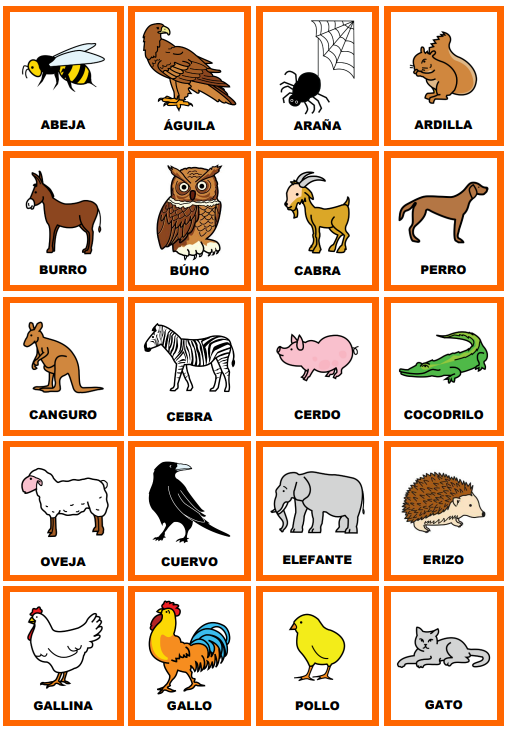
\includegraphics[width=0.4\textwidth]{figs/tablero_arasaac.png}
  \caption{Ejemplo de tablero de comunicación basado en pictogramas \ac{ARASAAC}.
  Fuente: \ac{ARASAAC} (\url{https://arasaac.org})}
  \label{fig:tablero_arasaac}
\end{figure}

\begin{itemize}
  \item \emph{Enunciados telegráficos.} Los usuarios tienden a emitir 
  secuencias reducidas de símbolos omitiendo elementos gramaticales funcionales como 
  artículos, preposiciones o morfemas flexivos.
  \item \emph{Orden de palabras no canónico.} La ausencia de morfología flexiva obliga 
  a interpretar el orden de las palabras. El protocolo de Soto evalúa específicamente 
  la presencia del orden Sujeto-Verbo-Objeto (\ac{SVO}).
  \item \emph{Omisión de morfología gramatical.} Dado que los pictogramas suelen 
  representar formas de cita (infinitivos, sustantivos sin flexión), la concordancia de 
  género, número, tiempo y aspecto puede estar ausente o ser asistida por el propio 
  dispositivo.
  \item \emph{Vocabulario restringido al conjunto disponible.} El léxico accesible depende 
  del vocabulario programado en el dispositivo, lo que puede diferir del vocabulario activo 
  real del usuario y sesgar los análisis basados en diversidad léxica.
\end{itemize}

Estos rasgos implican que los modelos y herramientas de \ac{PLN} entrenados sobre corpus
de habla típica no son directamente aplicables al lenguaje asistido sin adaptación
previa. El lenguaje producido por estos usuarios constituye un tipo de texto distinto al 
habla conversacional estándar, telegráfico y restringido por el vocabulario del dispositivo.
Esta constatación justifica que el sistema propuesto aquí no se limite al canal auditivo sino que
contemple también la información visual del vídeo de la sesión, si es posible.


\subsection{El Protocolo para el Análisis de Muestras de Lenguaje Asistido en SAAC}
\label{subsec:paalss}

El \textbf{\ac{PAALSS}} fue desarrollado por Gloria Soto, investigadora de la 
\emph{San Francisco State University}, como marco sistemático para evaluar el perfil 
lingüístico de personas que utilizan \ac{SAAC}~\cite{soto2020protocolo}. 
Un estudio piloto posterior de la propia autora~\cite{soto2024paalss_pilot} aplicó el 
protocolo de forma manual a una muestra de usuarios hispanohablantes, confirmando su 
viabilidad clínica pero constatando la elevada carga de trabajo del análisis manual, 
lo que refuerza la motivación del presente trabajo. El protocolo aborda el análisis 
desde cuatro dimensiones complementarias, cada una centrada en un nivel lingüístico 
diferente:

\begin{itemize}
  \item \emph{Vocabulario.} Se examina la diversidad léxica a partir de una lista de 219 
  palabras organizadas en categorías (sustantivos, verbos, adjetivos, pronombres y 
  palabras de función). La métrica principal es el número de tipos de palabras distintos 
  (\emph{number of different words}), complementada con la proporción de palabras nuevas 
  que el usuario introduce respecto a las que repite a lo largo de la muestra.

  \item \emph{Morfología.} Se analizan los morfemas gramaticales producidos en las dimensiones
  de género, número, tiempo verbal, aspecto y modo. Para cada morfema se registra si el
  usuario lo produce correctamente, lo omite o lo produce con error, lo que permite trazar 
  un perfil morfológico detallado del usuario.

  \item \emph{Complejidad gramatical.} Esta dimensión clasifica los enunciados en niveles de 
  complejidad creciente: desde palabras aisladas hasta cláusulas subordinadas. La métrica clave 
  es la \textbf{\ac{LME}}, calculada en morfemas o en palabras según la modalidad de análisis.

  \item \emph{Sintaxis.} Se evalúa la presencia y corrección del orden \ac{SVO}, la producción de 
  distintos tipos de oraciones (afirmativas, interrogativas, negativas) y el uso de 
  elementos relacionales como conjunciones o pronombres relativos.
\end{itemize}

Para la recogida de muestras, el protocolo recomienda un mínimo de 50 enunciados por
sesión, obtenidos en contextos naturales de interacción comunicativa.  La unidad de
análisis es el \emph{Communication Turn} (CT), definido como cada contribución que realiza
el usuario durante un turno de conversación.  El protocolo manual requiere que un
especialista en \ac{SAAC} transcriba la sesión, segmente los enunciados, los codifique
según las cuatro dimensiones y calcule las métricas globales.  Este proceso puede
extenderse varias horas por sesión, lo que constituye la principal barrera para su uso
sistemático en la práctica clínica y educativa~\cite{lsa_computer_programs}.


%% ============================================================
\section{Análisis automático de muestras de lenguaje}
\label{sec:lsa_automatico}
%% ============================================================

El análisis de muestras de lenguaje (\emph{Language Sample Analysis}, \ac{LSA}) es el
proceso de recoger, transcribir y cuantificar muestras de habla espontánea para obtener
indicadores objetivos del desarrollo o del perfil lingüístico de una persona. Se
considera el patrón de oro para evaluar las habilidades comunicativas expresivas, ya que
refleja el uso real del lenguaje en contextos naturales con mayor validez que las pruebas 
estandarizadas~\cite{lsa_computer_programs}.


\subsection{Herramientas clásicas: SALT, CLAN y SUGAR}
\label{subsec:salt_clan}

Los tres programas más utilizados en el contexto anglosajón para el LSA clínico: \textbf{\ac{SALT}}
(\emph{Systematic Analysis of Language Transcripts}), \textbf{\ac{CLAN}} (\emph{Computerized Language
Analysis}) y \textbf{\ac{SUGAR}} (\emph{Sampling Utterances and Grammatical Analysis Revised}),
aplicados a dos estudios de caso con niños preescolares \cite{lsa_computer_programs}.

\textbf{\ac{SALT}} es un software que calcula automáticamente métricas de producción lingüística a
partir de transcripciones en su propio formato anotado. Entre las métricas que computa
se incluyen la \ac{LME} en palabras y morfemas, el número de tipos léxicos distintos, la
tasa de disfluencias (\emph{mazes} o la proporción de elementos no fluidos en la producción 
del hablante) y el número de enunciados por minuto, y dispone de bases de datos normativas 
en inglés y español para distintos contextos comunicativos. Sin embargo, exige que el clínico 
proporcione la transcripción ortográfica completa y codifique manualmente las anotaciones 
morfológicas en una sintaxis propia, proceso que requiere formación específica y consume tiempo 
considerable~\cite{lsa_morphological_auto}.

\textbf{\ac{CLAN}} es la herramienta de análisis del sistema \textbf{\ac{CHILDES}} (\emph{Child Language Data
Exchange System}), que utiliza el formato de transcripción \textbf{\ac{CHAT}} (\emph{Codes for the
Human Analysis of Talk}). A diferencia de \ac{SALT}, \ac{CLAN} identifica automáticamente los
morfemas gramaticales con una precisión media del 94\%, sin necesidad de codificación
manual, e incluye módulos para el análisis morfosintáctico que permiten contrastar los resultados 
con \textbf{\ac{KIDEVAL}}, una base de datos normativa derivada de los corpus CHILDES con aproximadamente 
450 niños de desarrollo típico. 

\textbf{\ac{SUGAR}}, por su parte, no es un programa independiente sino un protocolo de codificación 
sobre un procesador de texto convencional: omite la codificación de morfemas y rellenos, lo que lo 
convierte en el más rápido de los tres (entre 18 y 22 minutos de codificación por muestra de 50 enunciados 
en los casos analizados por los autores), a costa de no detectar errores gramaticales ni calcular 
morfemas automáticamente.

Ninguno de los tres programas resulta adecuado para el lenguaje asistido por \ac{SAAC} para 
este proyecto: sus bases de datos normativas se construyeron sobre habla oral de niños con 
desarrollo típico, sin contemplar la ausencia de morfología en los pictogramas, el componente
gestual y multimodal ni el telegrafismo estructural propios del lenguaje
asistido, así como la barrera del idioma, ya que estas base de datos 
solo existen para el inglés y está construida sobre muestras de niños con desarrolo oral típico, 
sin \ac{SAAC} \cite{lsa_computer_programs}. Esta carencia es precisamente la que motivó el desarrollo 
del protocolo \ac{PAALSS} por parte de Gloria Soto.


\subsection{Automatización del pipeline de análisis}
\label{subsec:batchalign}

El trabajo más completo publicado hasta la fecha sobre la automatización integral del
\ac{LSA} es \emph{Batchalign}~\cite{lsa_automation_jslhr}. El sistema encadena siete módulos 
secuenciales:

\begin{enumerate}
  \item \emph{Reconocimiento automático del habla} (\ac{ASR}, \emph{Automatic Speech 
  Recognition}) mediante Rev~AI, con tasas de error de palabra (\emph{Word Error 
  Rate}, \ac{WER}) del 2{,}4--3{,}4\% en habla adulta.
  \item \emph{Segmentación en enunciados} mediante un modelo \ac{BERT} que predice los 
  límites de turno sobre la transcripción en crudo; alcanza una F1 del 86{,}9\%.
  \item \emph{Corrección automática} de la transcripción generada por el \ac{ASR}.
  \item \emph{Identificación de hablantes} o \emph{speaker diarization}.
  \item \emph{Alineación forzada} a nivel de palabra mediante el \emph{Montreal Forced 
  Aligner} (\ac{MFA}), que asigna marcas temporales a cada token.
  \item \emph{Corrección humana} de los errores residuales.
  \item \emph{Análisis morfosintáctico} automático mediante los módulos de \ac{CLAN}.
\end{enumerate}

\emph{Batchalign} reduce el tiempo de transcripción humana en un 75\% respecto al proceso
completamente manual, manteniendo una calidad comparable con la anotación experta. No
obstante, el sistema está diseñado para inglés y corpus de habla típica adulta, por lo
que su transferencia directa a lenguaje asistido en español requiere adaptación
sustancial y validación del proceso.


%% ============================================================
\section{PLN aplicado a lenguaje atípico}
\label{sec:pln_atipico}
%% ============================================================

El \ac{PLN} ha sido aplicado progresivamente al análisis de lenguaje producido en
condiciones no estándar: habla infantil, lenguaje de aprendices de segunda lengua,
habla de personas con trastornos neurológicos y comunicación asistida. Esta sección
revisa los avances más relevantes para este trabajo.


\subsection{Modelos de lenguaje y análisis morfosintáctico en español}
\label{subsec:pln_espanol}

Para el análisis morfosintáctico del español existen varias herramientas de referencia.
\emph{spaCy}~\cite{lsa_swiss_benchmark} ofrece modelos estadísticos y de redes neuronales para
el etiquetado \ac{POS}, el análisis de dependencias y el reconocimiento de entidades.

\emph{BETO}~\cite{beto_morphological} es un modelo tipo \emph{BERT} preentrenado sobre el corpus
\emph{BooksCorpus} en español más la Wikipedia española (3~GB), que ha demostrado mejorar el
rendimiento en tareas de clasificación de secuencias, etiquetado de secuencias y análisis
sintáctico en español respecto a los modelos multilingües.

Para el etiquetado \ac{POS} del habla espontánea en español,~\cite{spoken_spanish_pos}
se publicó COSER-PoS, un conjunto de datos de referencia anotado manualmente sobre
transcripciones de habla oral espontánea que permite evaluar sistemáticamente los
modelos existentes en condiciones de habla no formal, más cercanas al lenguaje asistido
que los corpus de texto escrito.  La evaluación reportada muestra que spaCy alcanza 
una exactitud (\emph{accuracy}) de entre 0{,}90 y 0{,}93 sobre habla oral, 
frente al 0{,}98--0{,}99 que obtienen sobre el corpus \emph{AnCora} de texto escrito,
lo que evidencia una caída de rendimiento sistemática al pasar de texto formal a habla
espontánea.

La naturaleza del lenguaje asistido plantea retos adicionales para estos modelos: 
la ausencia de morfología flexiva, el orden de palabras atípico y el vocabulario
reducido dan lugar a estructuras que se alejan de la distribución estadística de los
corpus de entrenamiento. Esto sugiere la necesidad de estrategias de adaptación al
dominio (\emph{domain adaptation}) o de enfoques con pocos ejemplos (\emph{few-shot}).


\subsection{PLN en contextos clínicos de lenguaje atípico}
\label{subsec:pln_clinico}

La aplicación de \ac{PLN} a la caracterización del lenguaje en poblaciones con trastornos
del neurodesarrollo ha avanzado considerablemente en la última década. Se ha demostrado 
que ciertas métricas lingüísticas calculadas automáticamente sobre transcripciones son 
sensibles a las diferencias en el patrón de lenguaje del \ac{TEA} \cite{nlp_autism_automated}. 
También se pudo demostrar que modelos estadísticos simples entrenados sobre datos clínicos 
limitados pueden replicar con precisión casi perfecta las anotaciones morfológicas de un 
experto \cite{lsa_morphological_auto}.

Se han identificado tres retos específicos del LSA en poblaciones pediátricas \cite{lsa_swiss_benchmark}: 

\begin{enumerate}
  \item La alta variabilidad inter e intrasujeto en pronunciación y vocabulario.
  \item La presencia de estructuras agramaticales o incompletas que confunden los modelos \ac{POS}.
  \item La escasez de datos anotados en habla infantil clínica, que impide el ajuste fino 
  (\emph{fine-tuning}) de modelos grandes
\end{enumerate}


%% ============================================================
\section{Aprendizaje con pocos ejemplos en PLN clínico}
\label{sec:fewshot}
%% ============================================================

Uno de los principales obstáculos para aplicar \ac{PLN} a dominios clínicos
especializados es la \textbf{escasez de datos etiquetados}: las anotaciones requieren
conocimiento experto costoso y tiempo considerable, mientras que las restricciones de
privacidad y la rareza de las condiciones estudiadas limitan la disponibilidad de
\emph{corpus} públicos. En el caso del lenguaje asistido por \ac{SAAC} en español esta
restricción es especialmente severa: no existe ningún corpus anotado
morfosintácticamente de acceso público, y la anotación del protocolo \ac{PAALSS}
requiere un especialista con formación específica en \ac{SAAC}. El aprendizaje con
pocos ejemplos (\emph{few-shot learning}) es la familia de técnicas que aborda
precisamente este escenario, permitiendo aprovechar modelos de lenguaje preentrenados
con una supervisión adicional mínima.

En el caso del lenguaje asistido por \ac{SAAC}, la escasez de datos se agrava por la
naturaleza misma del canal de comunicación: los pictogramas siempre representan la
\textbf{forma de cita} (infinitivo para los verbos, singular para sustantivos y adjetivos),
por lo que la información morfológica flexiva nunca está codificada explícitamente en
el texto producido. El sistema debe inferir, a partir del contexto conversacional, si
una forma como \emph{comer} corresponde a un presente habitual, a un imperativo o a
una referencia temporal pasada. Esta ambigüedad sistemática requiere un clasificador
capaz de operar con un número muy reducido de ejemplos anotados por un especialista
en \ac{SAAC}, lo que sitúa el aprendizaje con pocos ejemplos como la estrategia
natural para este dominio.

En el contexto de los modelos de lenguaje basados en \emph{Transformer}, pueden
distinguirse dos estrategias principales. El \emph{in-context learning} consiste en
incluir directamente en el \emph{prompt} varios ejemplos del formato \textbf{entrada-etiqueta}
y dejar que el modelo infiera el patrón sin actualizar ningún parámetro; esta
estrategia es característica de los modelos generativos de gran escala (\ac{LLM} de
centenares de miles de millones de parámetros) y resulta difícil de aplicar de forma
local por sus requisitos computacionales. Por otro lado, el ajuste fino
(\emph{fine-tuning}) sobre un conjunto reducido de ejemplos puede causar
sobreajuste y degradar las representaciones aprendidas durante el preentrenamiento,
en especial cuando solo se dispone de decenas de instancias por clase. Entre ambos
extremos, los métodos de aprendizaje con pocos ejemplos basados en modelos de lenguaje
enmascarado (\emph{Masked Language Model}, \ac{MLM}) ofrecen un equilibrio adecuado
para dominios clínicos de pequeño volumen.

El modelo \emph{BETO}~\cite{beto_morphological} es un modelo de tipo \emph{BERT}
preentrenado sobre más de 3 GB de texto en español procedentes de la Wikipedia y del
corpus \emph{BooksCorpus}, lo que lo convierte en la referencia para tareas de \ac{PLN}
en español que requieren comprensión morfológica y sintáctica profunda. \emph{BETO} ha
demostrado superar a los modelos multilingües en tareas de clasificación, etiquetado y
análisis sintáctico sobre el español, y resulta especialmente apropiado para el análisis
del lenguaje asistido porque su arquitectura de tipo \ac{MLM} admite la incorporación
de plantillas de clasificación con muy pocos ejemplos.

El método \textbf{\ac{PET}} (\emph{Pattern-Exploiting Training})~\cite{fewshot_clinical_nlp}
reformula la tarea de clasificación como un problema de modelado de lenguaje enmascarado:
dado un texto de entrada, se construye una plantilla (\emph{pattern}) que inserta el
texto en una oración incompleta, y se designa un verbalizador (\emph{verbalizer}) que
mapea las etiquetas de clase a \emph{tokens} concretos del vocabulario del modelo. El modelo
predice el \emph{token} más probable en la posición \texttt{[MASK]} y la clase predicha es la
etiqueta correspondiente al \emph{token} ganador. Este enfoque no requiere modificar la cabeza
de clasificación del modelo: se aprovecha directamente la distribución de probabilidad
del \ac{MLM} sobre el vocabulario del modelo base. Cuando se dispone de varios patrones
alternativos para una misma tarea, los predicciones de cada plantilla se combinan
mediante un proceso de destilación en un clasificador suave, lo que reduce la varianza
debida a la elección de una única plantilla.

Los resultados reportados en un entorno clínico de recursos limitados son altamente relevantes 
para este trabajo~\cite{fewshot_clinical_nlp}: con tan solo 20 ejemplos anotados por clase, 
\ac{PET} aplicado sobre un modelo \emph{BERT} adaptado al dominio médico eleva la precisión 
de la clasificación del 46\% al 79{,}1\% obtenida con un clasificador supervisado convencional 
sobre el mismo número de ejemplos. Esta ganancia de 33 puntos porcentuales con igual volumen de supervisión 
respalda la adopción de \ac{PET} sobre \emph{BETO} para el análisis de las categorías
morfológicas del lenguaje asistido en español, donde el número de ejemplos anotados
disponibles es del mismo orden de magnitud.

Estos resultados se alinean con la observación de Gorman~\cite{lsa_morphological_auto},
en los que se demostró que sistemas de reglas simples pueden superar al aprendizaje
automático supervisado cuando el \emph{corpus} de entrenamiento es reducido, y que la
combinación de reglas con modelos estadísticos permite alcanzar una precisión cercana
a la del anotador experto. Por este motivo, el sistema propuesto en este trabajo adopta
un enfoque híbrido: las categorías morfológicas con criterios explícitos, como la
distinción entre nombre y verbo en pictogramas de función semántica inequívoca, se
resuelven mediante heurísticos basados en el vocabulario \ac{ARASAAC}, reservando
\ac{PET} sobre \emph{BETO} únicamente para las categorías que presentan \textbf{ambigüedad
dependiente del contexto}, como la modalidad verbal o el tiempo gramatical inferido a
partir del enunciado del interlocutor.

%% ============================================================
\section{Generación Aumentada por Recuperación (RAG)}
\label{sec:ia_protocolos}
%% ============================================================

La \textbf{Generación Aumentada por Recuperación} (\ac{RAG}, \emph{Retrieval-Augmented Generation}) es
un paradigma de arquitectura de \ac{IA} generativa que combina un modelo de lenguaje (\ac{LLM}) con
un mecanismo de recuperación de información sobre una colección de documentos externa al
propio modelo. Frente a un \ac{LLM} de propósito general, que responde únicamente a partir
del conocimiento codificado durante su preentrenamiento, un sistema \ac{RAG} ancla cada
respuesta en fragmentos de texto recuperados de un documento concreto, lo que reduce de
forma sustancial las confabulaciones: respuestas plausibles pero incorrectas que mezclan
información de distintas fuentes vistas durante el entrenamiento~\cite{rag_lewis2020}.
Este paradigma resulta especialmente útil en tareas de extracción de información sobre
documentos extensos y de dominio específico, donde la respuesta a una pregunta concreta
existe en el documento pero localizarla manualmente requiere leer y comprender el texto
completo.

La arquitectura de un sistema \ac{RAG} se organiza habitualmente en cuatro fases.
En primer lugar, el documento se segmenta en fragmentos (\emph{chunks}) de tamaño
manejable, normalmente con cierto solapamiento entre fragmentos consecutivos para
preservar el contexto en los límites de cada segmento. A continuación, cada fragmento
se vectoriza mediante un modelo de \emph{embeddings} de frases y se almacena en una
base de datos vectorial que permite la búsqueda eficiente por similitud semántica; en
implementaciones locales se emplea habitualmente \emph{FAISS}
(\emph{Facebook AI Similarity Search}), una biblioteca de código abierto optimizada
para la búsqueda por vecinos más próximos en espacios vectoriales de alta dimensión.
Para cada consulta o campo a rellenar, una etapa de recuperación (\emph{retrieval})
extrae los $k$ fragmentos más similares mediante similitud coseno entre el
\emph{embedding} de la consulta y los del documento. Por último, el \ac{LLM} recibe
un \emph{prompt} estructurado con los fragmentos recuperados como contexto y genera la
respuesta fundamentada exclusivamente en ellos, con la instrucción explícita de señalar
la ausencia de información cuando los fragmentos recuperados no contengan la respuesta.

La viabilidad de esta arquitectura para la extracción de información en protocolos
clínicos ha sido validada empíricamente por Babaeipour~\cite{clinical_nlp_ai_protocol}: en este
estudio se comparó un \ac{LLM} autónomo con un sistema \ac{RAG} sobre la tarea de
extraer información estructurada de protocolos de ensayos clínicos, y el enfoque \ac{RAG}
alcanzó una exactitud del 89\% frente al 62{,}6\% del \ac{LLM} sin recuperación,
reduciendo además de forma sustancial las confabulaciones (\emph{hallucinations}).
Estos resultados confirman que anclar la generación en fragmentos recuperados del
documento de referencia es la estrategia adecuada cuando se requiere que las respuestas
sean trazables y verificables, una propiedad imprescindible en un sistema de asistencia
a la cumplimentación de un protocolo clínico como el \ac{PAALSS}.

En el contexto de este trabajo, la restricción de procesamiento local impuesta por el
\ac{RGPD} descarta el uso de \ac{LLM} accesibles únicamente a través de \ac{API}
externas. La herramienta \emph{Ollama}~\cite{ollama} permite ejecutar localmente
modelos de la familia \emph{Llama} y similares sin ejecutarlos en la nube, ofreciendo una
interfaz de \ac{API} compatible con los estándares habituales de integración, lo que
facilita la sustitución del modelo por versiones más actualizadas a medida que la
investigación avance.


%% ============================================================
\section{Transcripción automática y análisis multimodal}
\label{sec:transcripcion_multimodal}
%% ============================================================

Los avances recientes en reconocimiento automático del habla (\ac{ASR}) y en la
combinación de \ac{ASR} con diarización de hablantes abren la posibilidad de procesar
directamente las grabaciones de vídeo de las sesiones de comunicación asistida.


\subsection{Reconocimiento automático del habla con Whisper}
\label{subsec:whisper}

\emph{Whisper}~\cite{whisper_radford2023} es un modelo \ac{ASR} desarrollado por
\emph{OpenAI} basado en la arquitectura \emph{Transformer encoder-decoder},
preentrenado mediante supervisión débil a gran escala: los 680.000 horas de audio de
entrenamiento proceden de Internet y se emparejan automáticamente con sus
transcripciones en múltiples idiomas, lo que elimina la necesidad de anotación manual
masiva y dota al modelo de una capacidad de generalización notable sobre acentos, ruido
de fondo y registros informales~\cite{whisper_radford2023}. El modelo es capaz de
transcribir y traducir hasta 98 idiomas, incluyendo el español, y supera o iguala el
estado del arte en varios \emph{benchmarks} de robustez sin ajuste fino específico.

El modelo existe en varias configuraciones de tamaño: \texttt{tiny} (39~M parámetros),
\texttt{base} (74~M), \texttt{small} (244~M), \texttt{medium} (769~M) y \texttt{large}
(1.550~M). La variante \texttt{small} ha demostrado ser un compromiso adecuado entre
precisión y coste computacional en aplicaciones de análisis del lenguaje clínico que
requieren despliegue local~\cite{lsa_swiss_benchmark,whisper_diarization_realtime},
mientras que la variante \texttt{large-v3} ofrece la mayor exactitud disponible y
resulta adecuada cuando el equipo dispone de \ac{GPU} con al menos 6~GB de VRAM. Para
el despliegue local eficiente se emplea \texttt{faster-whisper}, una reimplementación
de \emph{Whisper} en \emph{CTranslate2} que reduce el consumo de memoria mediante
cuantización en coma flotante de 16 bits y permite ejecutar el modelo \texttt{large-v3}
en \ac{GPU} con un consumo inferior a 6 GB de VRAM.

Un aspecto relevante para las sesiones de comunicación asistida es que la voz
producida por el dispositivo generador de voz (\ac{TTS}) del comunicador electrónico
difiere acústicamente de la voz humana natural: es más uniforme, sin variaciones de
entonación ni disfluencias. \emph{Whisper} transcribe correctamente los fragmentos de
\ac{TTS}, pero los modelos de diarización pueden tender a asignar estos fragmentos al clúster
del interlocutor adulto en lugar de al usuario del \ac{SAAC}, lo que requiere un
postprocesado específico descrito en el capítulo de metodología.


\subsection{Diarización de hablantes}
\label{subsec:diarizacion}

En las sesiones de comunicación asistida intervienen típicamente al menos dos
participantes: el usuario del \ac{SAAC} y el interlocutor. Para el análisis del protocolo
\ac{PAALSS} es necesario atribuir cada enunciado al hablante correcto, lo que requiere
diarización (\emph{speaker diarization}): la tarea de segmentar el audio y etiquetar cada
segmento con la identidad del hablante.

Existen distintos enfoques para abordar esta tarea. Un primer enfoque combina \emph{Whisper} con
un modelo de \emph{embedding} de hablante y \emph{clustering} incremental sobre los propios
segmentos de la transcripción~\cite{whisper_diarization_realtime}, pensado para
funcionar en tiempo real con un número variable de hablantes, condiciones que no exige el
análisis \ac{PAALSS}, realizado \emph{a posteriori} sobre grabaciones de dos hablantes
fijos. Un segundo enfoque, \textbf{DiCoW} (\emph{Diarization-Conditioned Whisper}),
condiciona el \emph{encoder} de Whisper con la salida de un diarizador externo mediante
máscaras STNO y mecanismos de \emph{Query-Key Biasing} y \emph{Frame-Level
Diarization-Dependent Transformations}~\cite{dicow_diarization}, evitando así el
enrolamiento del hablante objetivo, aunque requiere una etapa externa de diarización y un
ajuste fino sobre corpus en inglés alejados de las condiciones acústicas de una sesión
infantil en español. Un tercer enfoque, \emph{pyannote.audio}~\cite{pyannote_plaquet2023}, es una
herramienta de propósito general que no requiere ajuste fino ni enrolamiento y se
distribuye como \emph{pipeline} preentrenado de uso directo, lo que la hace adecuada
para escenarios fijos de dos hablantes sin restricciones de latencia. Su arquitectura
combina segmentación a nivel de \emph{frame}, extracción de \emph{embeddings} de
hablante y \emph{clustering} jerárquico aglomerativo, y está implementada como
librería Python de código abierto con modelos preentrenados disponibles en
\emph{HuggingFace}.


%% ============================================================
\section{Síntesis comparativa}
\label{sec:comparativa}
%% ============================================================

La revisión realizada en este capítulo pone de manifiesto que los trabajos existentes
abordan componentes aislados del problema pero ninguno integra todos los elementos
necesarios para la automatización del protocolo \ac{PAALSS} en español: la extracción
de enunciados desde vídeo, el procesamiento morfosintáctico del lenguaje asistido, el
cálculo de las métricas del protocolo y el pre-rellenado del formulario clínico. La
Tabla~\ref{tab:comparativa} resume las principales herramientas y enfoques revisados
en relación con las dimensiones más relevantes para este trabajo.

\begin{table}[h]
  \footnotesize
  \renewcommand{\arraystretch}{1.3}
  \setlength{\tabcolsep}{4pt}
  \begin{center}
  \begin{tabular}{|L{2.1cm}|C{1.4cm}|C{1.7cm}|C{1.4cm}|C{1.3cm}|C{1.2cm}|L{4.0cm}|}
  \hline
  \rowcolor{tema!10}
  \bft{Herramienta} & \bft{Idioma} & \bft{Entrada} & \bft{Transcr.\ auto.} & \bft{Morfol.\ auto.} & \bft{Adapt.\ SAAC} & \bft{Limitación principal} \\ \hline
  SALT & EN / ES & Texto manual & No & Parcial & No &
  Requiere transcripción y codificación manual; bases de datos normativas solo en inglés \\ \hline
  CLAN / Batchalign & EN & Texto / Audio & Sí & Sí & No &
  Diseñado para habla oral típica en inglés; no contempla pictogramas ni lenguaje telegráfico \\ \hline
  SUGAR & EN & Texto manual & No & No & No &
  Método manual simplificado; no detecta errores gramaticales ni calcula morfemas \\ \hline
  LLUNA & EN & Texto manual & No & Parcial & No &
  Limitado a narrativas; sin componente multimodal ni adaptación al español \\ \hline
  Medidas LSA/TEA & EN & Texto manual & No & Sí & No &
  Diseñado para \ac{TEA}; no adaptado a \ac{SAAC} ni al español \\ \hline
  Benchmark PLN infantil & DE/FR/\,IT & Texto & No & Sí & No &
  Habla infantil típica en lenguas suizas; sin canal de vídeo ni lenguaje asistido \\ \hline
  \rowcolor{tema!10}
  \bft{Este trabajo} & \bft{ES} & \bft{Vídeo} & \bft{Sí} & \bft{Sí} & \bft{Sí} &
  Validado sobre una única usuaria; canal visual (pictogramas) pendiente de implementar \\ \hline
  \end{tabular}
  \end{center}
  \caption[Comparativa de herramientas]{Comparativa de herramientas y enfoques de análisis automático del lenguaje.}
  \label{tab:comparativa}
  \renewcommand{\arraystretch}{1}
\end{table}

De la comparativa se extraen tres conclusiones que fundamentan las decisiones de diseño
del sistema propuesto. En primer lugar, todas las herramientas existentes para el
\ac{LSA} automático operan sobre texto ya transcrito, sin abordar la extracción de
enunciados desde vídeo, lo que constituye la diferencia más radical del presente
trabajo. En segundo lugar, ninguna herramienta revisada ha sido diseñada o adaptada
para el lenguaje asistido por \ac{SAAC}, lo que implica que las métricas calculadas
sobre habla oral típica no son directamente transferibles. En tercer lugar, la barrera
del idioma es un obstáculo transversal: todos los sistemas con automatización completa
están diseñados y validados para el inglés, lo que justifica la elección de modelos
específicos para el español como \emph{BETO} y \texttt{es\_core\_news\_lg} y la
restricción del alcance del trabajo a una única lengua.
 

% Objetivos
\chapter{Objetivos}
\label{chap:objetivos}

\section{Objetivo general}

El análisis de muestras de lenguaje (\emph{Language Sample Analysis}, \ac{LSA}) constituye el
patrón de referencia para la evaluación expresiva en intervención logopédica, y el
protocolo para el análisis de muestras de lenguaje asistido por \ac{SAAC}, definido por Gloria
Soto~\cite{soto2020protocolo}, traslada esa metodología al caso de los usuarios de
Sistemas de Comunicación Aumentativa y Alternativa (\ac{SAAC}). Su aplicación manual exige
segmentar y codificar al menos cincuenta enunciados a lo largo de cuatro dimensiones, 
lo que se traduce en un coste de varias horas de trabajo profesional por sesión grabada. 
Este coste temporal limita en la práctica la frecuencia con la que los especialistas pueden 
aplicar el protocolo, y motiva la búsqueda de un sistema que reduzca dicha carga sin sustituir 
el juicio clínico del profesional.

El objetivo general de este trabajo es diseñar e implementar un prototipo de
automatización parcial del protocolo \ac{PAALSS} centrado en el \textbf{canal auditivo}
de la sesión, mediante modelos de \ac{IA} y \ac{PLN} que reduzcan la carga de trabajo
manual del especialista. El sistema actúa como asistente de pre-anotación: propone
valores para las métricas del protocolo a partir del procesamiento del audio de la
sesión, mientras que la validación final recae siempre en el profesional, sin que el
sistema emita diagnóstico alguno ni sustituya el juicio clínico experto. El análisis
del canal visual así como del registro del dispositivo (selección de pictogramas y gestos) 
se plantea como extensión futura del prototipo, una vez validado el canal auditivo sobre 
las sesiones disponibles.

Ningún trabajo previo revisado en el estado del arte aborda esta automatización para el
protocolo \ac{PAALSS}. Los precedentes más cercanos operan sobre transcripciones ya elaboradas, 
en inglés y sin componente multimodal, por lo que no resuelve ni la extracción de enunciados
desde vídeo ni el pre-rellenado de un formulario clínico estructurado en español. Del
mismo modo, las herramientas de \ac{LSA} automático de mayor difusión (Batchalign, 
\ac{SALT}, \ac{CLAN}) se han desarrollado y validado sobre el inglés, y los modelos de \ac{PLN} 
disponibles para el español, como \emph{BETO} o \emph{spaCy-es}, degradan su rendimiento sobre 
habla espontánea e infantil. Esta ausencia de precedente directo justifica el planteamiento de los
cuatro objetivos específicos que se describen a continuación.

Por último, cabe destacar que el sistema se concibe bajo una restricción de procesamiento
local: dado que los datos manejados corresponden a sesiones de menores con discapacidad,
ninguna fase del \emph{pipeline} puede depender de servicios en la nube. 
Esta restricción condiciona de forma transversal el diseño de todos los objetivos específicos y, 
en particular, la elección de las tecnologías empleadas en cada módulo.

\section{Objetivos específicos}

A partir del objetivo general, se han definido cuatro objetivos específicos que
cubren de forma secuencial las fases necesarias para construir el sistema: extracción de
enunciados desde el canal auditivo del vídeo, procesamiento lingüístico de dichos
enunciados, clasificación morfológica de las categorías ambiguas propias del lenguaje
asistido, y generación automática del pre-rellenado del formulario. Cada uno de ellos
responde a una carencia concreta detectada en la revisión del estado del arte.

\subsection{OE1: Extracción automática de enunciados}

Implementar un sistema automático de extracción de enunciados desde el canal auditivo del
vídeo de la sesión, mediante transcripción automática del habla, diarización de hablantes
y fusión de ambas señales en Turnos Comunicativos (CT) atribuidos al hablante
correspondiente. La transcripción se apoya en modelos \emph{Whisper}~\cite{whisper_radford2023}
ejecutados de forma local mediante \texttt{faster-whisper}, mientras que la diarización
separa los turnos de la persona usuaria de SAAC de los de su interlocutor mediante
enfoques como \emph{pyannote.audio}~\cite{pyannote_plaquet2023} o
\emph{DiCoW}~\cite{dicow_diarization}.
El análisis de la modalidad visual, selección de pictogramas, gesto y mirada, queda planteado
como línea de trabajo futuro, una vez implementado la solución para el canal auditivo.

\subsection{OE2: Pipeline de procesamiento lingüístico}

Diseñar un \emph{pipeline} de procesamiento lingüístico que identifique \textbf{categorías
gramaticales}, \textbf{estructuras morfológicas} y \emph{patrones sintácticos} definidos en el 
protocolo de Gloria Soto, adaptando los modelos de \ac{PLN} disponibles para el español a las
particularidades del lenguaje producido con \ac{SAAC}. Estas particularidades incluyen el uso
de pictogramas en forma de cita (infinitivo, singular), la ausencia de inflexión
morfológica explícita en la selección y la naturaleza telegráfica de los enunciados. Dado
que herramientas como \emph{spaCy}~\cite{spoken_spanish_pos} o
\emph{BETO}~\cite{beto_morphological} se han entrenado sobre habla y texto estándar,
su aplicación directa requiere una capa de adaptación que tenga en cuenta el contexto
multimodal de la sesión y no únicamente la etiqueta léxica del pictograma.

\subsection{OE3: Modelos de análisis gramatical}

Desarrollar un clasificador de las categorías morfológicas ambiguas propias del
lenguaje asistido por pictogramas: aquellas que no pueden resolverse mediante el
etiquetado estándar de herramientas de \ac{PLN} entrenadas sobre habla oral, porque
el contexto comunicativo del \ac{SAAC} altera el valor morfológico esperado de la
forma de cita. La estrategia adoptada combina reglas lingüísticas explícitas para
los casos deterministas con clasificación \emph{zero-shot} mediante el modelo de
lenguaje \emph{BETO}~\cite{beto_morphological} y \emph{Pattern-Exploiting
Training}~\cite{fewshot_clinical_nlp} para los casos en que el contexto es
necesario para dirimir la ambigüedad.

\subsection{OE4: Módulo de pre-rellenado del protocolo}

Desarrollar un módulo que traduzca las métricas calculadas en OE2 y OE3 en propuestas
de valores para cada campo del formulario \ac{PAALSS}, de forma trazable y vinculada
a los enunciados que las sustentan. Sumado a esto, se propone una arquitectura de generación
aumentada por recuperación (\emph{Retrieval-Augmented Generation}, \ac{RAG})
\cite{rag_lewis2020} que recupera los \ac{CT} semánticamente relevantes para cada
campo mediante una base vectorial, y los emplea como contexto para un modelo de
lenguaje local que genera observaciones acerca de la sesión. Este \emph{RAG} no representa una 
arquitectura completa final, sino que se plantea como una primera versión parcial para un desarrollo
futuro. El resultado se exporta como \ac{PDF} editable del formulario oficial, de modo que el especialista pueda revisar,
corregir y validar cada campo propuesto sin necesidad de partir de cero.

\section{Alcance y limitaciones}

El presente trabajo se circunscribe al español y a los tableros de comunicación basados en
el catálogo de pictogramas de \textbf{\ac{ARASAAC}}, y se valida únicamente sobre dos sesiones
anotadas por expertos correspondientes a una misma usuaria, lo que condiciona la
generalización de los resultados a otros perfiles de usuario o a otros sistemas de
comunicación aumentativa. El sistema se limita, además, a la generación de un
pre-rellenado del protocolo y no constituye en ningún caso una herramienta de diagnóstico,
quedando la validación final del formulario siempre a cargo del profesional. El
procesamiento de la modalidad visual (selección de pictogramas, gesto y mirada) se
plantea como línea de trabajo futuro y queda fuera del alcance de esta primera versión, que
se centra en el canal auditivo de la sesión. Por último, y dado que los datos manejados
corresponden a menores con discapacidad, todo el procesamiento se ejecuta de forma local,
sin recurrir a servicios en la nube, lo que excluye del alcance del trabajo cualquier
modelo o API que requiera el envío de datos a terceros.

\section{Requisitos}

En cuanto a los requisitos \emph{funcionales}, se pueden enumerar los siguientes:

\begin{itemize}
  \item \emph{Extracción de enunciados}. El sistema debe generar, a partir de un vídeo de
  sesión, una lista de \textbf{Turnos Comunicativos} con su transcripción, su atribución de
  hablante y sus marcas temporales.
  \item \emph{Procesamiento lingüístico}. Cada \textbf{Turno Comunicativo} debe poder anotarse con
  sus categorías gramaticales, su estructura morfológica y su patrón sintáctico.
  \item \emph{Pre-rellenado del protocolo}. El sistema debe producir, para cada sesión
  procesada, un conjunto de métricas y tablas correspondientes a las cuatro dimensiones del
  protocolo \textbf{\ac{PAALSS}}, trazables hasta los enunciados que las originan.
  \item \emph{Exportación}. El resultado del pre-rellenado debe poder exportarse en un
  formato que permita su revisión y edición por parte del profesional.
\end{itemize}

Por otra parte, los requisitos \emph{no funcionales} considerados son los siguientes:

\begin{itemize}
  \item \emph{Procesamiento local}. Ninguna fase del sistema puede depender de servicios
  en la nube, en cumplimiento del Reglamento General de Protección de Datos (RGPD) y dado
  que los datos corresponden a menores con discapacidad.
  \item \emph{Trazabilidad}. Toda métrica generada debe poder vincularse al enunciado o
  conjunto de enunciados que la sustentan, de forma que el profesional pueda auditar el
  resultado propuesto por el sistema.
  \item \emph{Idioma}. El sistema debe operar sobre transcripciones y enunciados en
  español, incluyendo las variantes propias del habla infantil y del lenguaje asistido.
  \item \emph{Validez clínica}. El sistema no sustituye el juicio profesional; sus salidas
  se conciben como propuesta de pre-anotación sujeta a confirmación o corrección por parte
  del especialista. No hay validación con ninguna métrica, debido a la falta de muestras y
  que no entra en los objetivos de este análisis.
\end{itemize}

% Local Variables:
%  coding: utf-8
%  mode: latex
%  mode: flyspell
%  ispell-local-dictionary: "castellano8"
% End: 

% Algunos elementos
\chapter{Algunos elementos}

En este capítulo se describen algunas particularidades de la plantilla, y se proporcionan algunos ejemplos con elementos de uso frecuente. No se comentan aspectos comunes relacionados con el uso de \LaTeX, ya que existe gran cantidad de información al respecto.

\section{Configuración}
La configuración es muy sencilla. Al margen de la adaptación particular que pueda hacerse, la elaboración de un documento solamente requiere información relativa al autor, título y tutores. Ésta ha de configurarse en el archivo \verb+include\opciones.tex+.  \\

Además, en el archivo \verb+include\colores.tex+ puede configurarse el color \verb+tema+, utilizado en títulos, elementos flotantes y, opcionalmente, tablas y negritas. Por defecto, se recomienda ponerlo a \verb+{0,0,0}+  (negro). Pueden escribirse \bft{negritas con el color configurado} con el comando \verb+\bft{texto}+. \\

Por último, en el archivo principal se pueden configurar las fuentes utilizadas en la portada, preámbulo y documento.

\section{Colores}


En el archivo \verb+include\colores.tex+ se predefinen algunos colores. También varios comandos para utilizar negritas con ellos. En concreto, se proporcionan cinco: Con el comando \verb+\bfa{texto}+ se pueden poner las cosas en negrita \bfa{azul}. Con el comando \verb+\bfr{texto}+ se pueden poner las cosas en negrita \bfr{rojo}.Con el comando \verb+\bfn{texto}+ se pueden poner las cosas en negrita \bfn{naranja}. Con el comando \verb+\bfv{texto}+ se pueden poner las cosas en negrita \bfv{verde}. Con el comando \verb+\bfm{texto}+ se pueden poner las cosas en negrita \bfm{mostaza}. \\

\begin{itemize}
\item [\hmarkr] No es conveniente usar los colores salvo en alguna ocasión puntual. Por ejemplo, si el color del tema es {\bf negro} o \bfa{azul} se puede utilizar el \bfr{rojo} para alguna advertencia.
\end{itemize}

\section{Listas y enumeraciones}

El entorno \textit{itemize} usa, por defecto, el color del tema. Los símbolos utilizados para marcar los items están pre-definidos en el archivo de configuración, y pueden cambiarse. También es posible seleccionar, mediante \verb+\item[símbolo]+ el símbolo específico para cada línea. Esta lista muestra los símbolos por defecto:

\begin{itemize}
\item Primer ítem
\begin{itemize}
\item Primer ítem en el segundo nivel
\item Otro ítem en el segundo nivel
\begin{itemize}
\item Ítem en el tercer nivel
\end{itemize}
\end{itemize}
\item Segundo ítem
\item Tercer ítem \\
\end{itemize}

En esta se usan algunos caracteres especiales predefinidos para marcar los ítems. Existen comandos para mostrar algunos de estos caracteres con los colores azul, rojo y el color del tema.

\begin{itemize}
\item[\vmarka] \verb+\vmarka+ : ``v'' representa el símbolo, y ``a'' el color
\item[\xmarkr] \verb+\xmarkr+
\item[\lmarkt] \verb+\lmarkt+ : el color ``t'' corresponde al tema.
\item[\hmarkt] \verb+\hmarkt+ 
\item[\fmarkt] \verb+\fmarkt+ \\
\end{itemize}

Las enumeraciones también están preconfiguradas en el archivo de configuración:

\begin{enumerate}
\item Esto es una enumeración
\item Con algunos elementos adicionales
\item Que se pueden quitar
\end{enumerate}

Pueden ser modificadas, como en el siguiente ejemplo.

\begin{enumerate}[labelindent=\parindent ,leftmargin=*,label=\mbox{\bft{[Re \arabic*]}}]
\setcounter{enumi}{7}
\item Esto es una enumeración
\item Sin elementos
\item Adicionales
\end{enumerate}


\section{Elementos flotantes}

En el archivo de \verb+include\configuracion+ existen varios parámetros que se fijan en la configuración para figuras y tablas, pero se pueden alterar de manera ocasional (y excepcional) al maquetar el documento. La mayoría son relativos al título, y se pueden cambiar a través de las funcionalidades que proporciona el paquete \verb+caption+. Cuando se cambian para un elemento particular \bft{es buena práctica restaurar el valor original}, para que el documento tenga un aspecto uniforme.

\begin{verbatim}
% Títulos
\DeclareCaptionFont{tema}{\color{tema}} % Color
\captionsetup{labelfont={tema, bf}}     % Estilo
\captionsetup{font=normalsize}          % Tamaño
\captionsetup{width=.9\linewidth}       % Anchura del título
 % Distancia de la figura al texto.
\setlength{\intextsep}{1cm} 
\setlength{\textfloatsep}{1cm}         
\end{verbatim}

\subsection{Tablas}
Las tablas se hacen de modo normal, aunque se ha añadido la capacidad utilizar celdas que ocupen múltiples filas, colores en los encabezados, y anchuras fijas. Se recomienda mirar el código fuente de la tabla \ref{tab:mod1}.\\

Con respecto al color de los encabezados, es conveniente utilizar el mismo en todo el documento. Una opción con respecto al fondo del encabezado es utilizar el mismo que el del texto pero con transparencia. \\



% --------------------------------------------------
% Esto es para poner colores en las asignaturas
% en el ejemplo concreto
\newcommand{\bi}{\bfn{ES}/\bfr{EN}}
\newcommand{\esp}{\bfn{ES}}
\newcommand{\eng}{\bfr{EN}}
% --------------------------------------------------

\begin{table}[h]\footnotesize
\renewcommand{\arraystretch}{1.3} % Altura
\begin{center}
\begin{tabular}{|L{2.5cm}| L{3cm}| C{6cm} c | c |} % Tres primeras con anchura predefinida
\hline 

\rowcolor{tema!10} % Color con transparencia correspondiente
\hline
\bft{Módulo I} & \bft{Materia} & \multicolumn{2}{|c|}{\bft{Asignatura}}& \bft{ECTS} \\ \hline 
\multirow{9}{2.5cm}{Formación Básica (60 ECTS)} & % Aquí se indica que esta ocupa nueve filas.
\multirow{4}{3cm}{Fundamentos Matemáticos de la Informática} & 
Álgebra y Matemática Discreta & \esp  & 6 \\ \cline{3-5} 
& & Cálculo y Métodos Numéricos & \bi  & 6 \\ \cline{3-5} 
& & Estadística & \bi  & 6 \\ \cline{3-5}
& & Lógica& \esp  & 6 \\ \cline{2-5}
& Fundamentos Físicos de la Informática & Fundamentos Físicos de la Informática & \bi  & 6 \\ \cline{2-5}
& \multirow{2}{3cm}{Ingeniería de Computadores} & 
Estructura de Computadores & \esp  & 6 \\ \cline{3-5} 
& & Tecnología de Computadores & \esp  & 6 \\ \cline{2-5} 
& \multirow{2}{3cm}{Programación} & 
Fundamentos de Programación I & \esp  & 6 \\ \cline{3-5} 
& & Fundamentos de Programación II & \bi  & 6 \\ \cline{2-5}
%& \makecell[cl]{Gestión de las \\ Organizaciones} & Fundamentos de Gestión Empresarial & \esp  & 6 \\ \hline 
& Gestión de las \mbox{Organizaciones} & Fundamentos de Gestión Empresarial & \esp  & 6 \\ \hline 
\end{tabular}
\end{center}
\caption[Asignaturas del Módulo I]{Asignaturas del Módulo I.}
\label{tab:mod1}
\renewcommand{\arraystretch}{1} 
\end{table}

\subsection{Figuras}

Con respecto a las figuras, a veces es utilizar un texto descriptivo demasiado ancho puede ser antiestético. Por ejemplo en la \ref{fig:esiiabI} el rótulo ocupa toda la línea\footnote{Por defecto, ocupa el 90\%, que es el valor por defecto en la configuración, pero se ha cambiado para que se vea mejor el efecto.}. En la figura \ref{fig:esiiabII} se corrige este efecto con:

\begin{verbatim}
\begin{figure}[b] 
\captionsetup{width=0.8\linewidth}
...
\end{verbatim}

Después, se restaura el valor original de la configuración:
\begin{verbatim}
...
\captionsetup{width=0.9\linewidth}
\end{figure}
\end{verbatim}


\begin{figure}[p] 
\captionsetup{width=1\linewidth}
\begin{center}
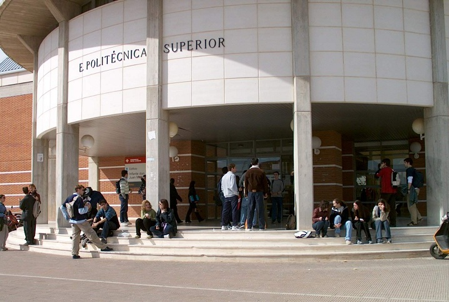
\includegraphics[width=10cm]{figs/esiiab.png}
\end{center}
\caption[Escuela Superior de Ingeniería Informática I]{Escuela Superior de Ingeniería Informática. Esto es un texto descriptivo algo más largo que puede producir un efecto feo.}
\label{fig:esiiabI}
\end{figure}



\begin{figure}[p] 
\captionsetup{width=0.8\linewidth}
\begin{center}
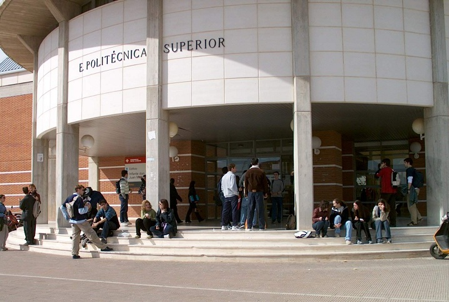
\includegraphics[width=10cm]{figs/esiiab.png}
\end{center}
\caption[Escuela Superior de Ingeniería Informática II]{Escuela Superior de Ingeniería Informática. Esto es un texto descriptivo algo más largo que puede producir un efecto feo.}
\label{fig:esiiabII}
\captionsetup{width=0.9\linewidth}
\end{figure}

Se incluye el paquete \verb+subfigure+ para la inclusión de figuras con varias imágenes o gráficas, como la que muestra la figura \ref{fig:subfiguras}.
\begin{figure}[htb]
\begin{center}
\begin{subfigure}[b]{0.4\linewidth}
\begin{center}
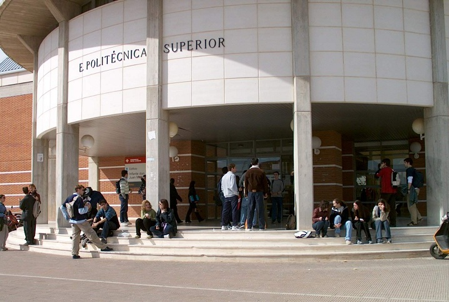
\includegraphics[width=0.9\linewidth]{figs/esiiab.png}
\caption{Fotografía de la izquierda}\label{fig:esiiabIII}
\end{center}
\end{subfigure} 
\begin{subfigure}[b]{0.4\linewidth}
\begin{center}
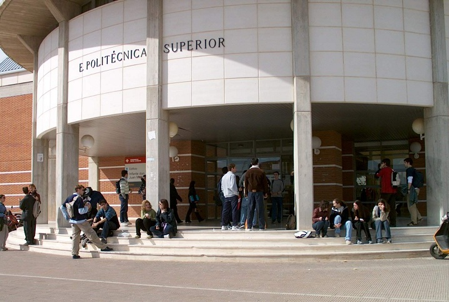
\includegraphics[width=0.9\linewidth]{figs/esiiab.png}
\caption{Fotografía de la drecha}\label{fig:esiiabIV}
\end{center}
\end{subfigure} 
\end{center}
\caption[Ejemplo de subfiguras]{Ejemplo de inclusión de subfiguras}
\label{fig:subfiguras}
\end{figure}



\section{Algoritmos y código}

Con respecto a los algoritmos (pseudocódigo) y código pueden implementarse, respectivamente, mediante el uso de los paquetes \verb+algorithmic+ y \verb+listings+. Pueden configurarse ambos entornos el archivo \verb+include\configuracion+. Por otra parte, se han definido dos entornos flotantes, denominados \verb+algorithm+ y \verb+code+ para encapsular y mostrar ambos tipos de elemento de manera uniforme.\\


El algoritmo \ref{alg:search} muestra un ejemplo de pseudocódigo. Se han añadido dos comandos, \verb+\va{variable}+ para distinguir las \va{variables}, y \verb+\fu{funcion}+ para distinguir las \fu{Funciones}. \\



\begin{algorithm}[b]
\begin{algorithmic}[1]
 	\Function{Tree-Search}{ }
 	\State \va{open} $\leftarrow$ \Call{CreateNode}{\fu{Initial-State}} \Comment{Creates the root}
	\While {\va{open} $\neq \emptyset$}
		\State \va{node} $\leftarrow$ \Call{Extract}{\va{open}}
		\If {\Call{TestGoal}{\va{node.STATE}}}
			\State \Return \Call{RecoverPath}{\va{node}} \Comment{Solution found}
		\EndIf		
				
		\State \va{successors} $\leftarrow$ \Call{Expand}{\va{node}}
		\ForAll {\va{successor} \bft{en} \va{successors}} \Comment{Processes each successor }
			\State  \Call{Insert}{\va{successor, open}}
		\EndFor	
	\EndWhile
	\State \Return failure \Comment{No solution have been found}
 	\EndFunction
\end{algorithmic}
\caption{Tree-Search exploration}
\label{alg:search}
\end{algorithm}

Por último, el listado \ref{alg:code} muestra el código del algoritmo \ref{alg:search} en \textit{Python}. El paquete \verb+listings+  contiene multitud de opciones para el manejo de distintos lenguajes y para personalización.

\begin{code}
\begin{lstlisting}

def search(initial):
	open = [initial]
	while open:
		node = open.pop()
		if testGoal(node):
			return recoverPath(node)
		successors = expand(node)
		for succesor in successors:
			open.append(succesor)
	return failure
		
\end{lstlisting}
\caption{Ejemplo de código en Python}
\label{alg:code}
\end{code}


\section{Bibliografía}

Esto es una cita \cite{RUSSELL} y esto otra \cite{AlphaZero}. La bibliografía se gestiona con bibtex y un estilo predefinido. No se han hecho modificaciones de momento.

\section{Notación matemática}

Utiliza las fuentes por defecto del tema, aunque también se pueden cambiar.


\[
J(\theta)=\frac{1}{2m}\left[ \sum_{i=1}^m\left(h_\theta(x^{(i)})-y^{(i)}\right)^2 + \lambda \sum_{j=1}^n \theta_j^2 \right], \mbox{ } \lambda >0
\]

 

% Utilidades para anotaciones
\input{chapters/ch3} 

% -------------------------------
% Apéndices
% -------------------------------
\appendix
\chapter{Anexo 1}
\lipsum[1-2]

\cleardoublepage
\thispagestyle{empty}


% -------------------------------
% Bibliografía
% -------------------------------
\bibliographystyle{apalike}
\bibliography{bib/ref} 
\addcontentsline{toc}{chapter}{Referencia bibliográfica} % Añade a la tabla de contenidos

\end{document}